\section{微分}

本节给出微分概念。
着重理解微分及其意义和工程应用。

本节要点:
\begin{itemize}
    \item 熟练掌握微分概念;
    \item 学会推导微分定理。
\end{itemize}

~

工程上,经常碰到已知$f\left( x_0 \right) $,求$f\left( x_0+\Delta x \right) $的问题。
这个问题在数学上就是$\Delta y$能不能通过$\Delta x$的线性计算获得,误差多少,即:
\[
\Delta y=A\Delta x+B\left( \Delta x \right)
\]
且我们希望$A$与$\Delta x$无关,$B\left( \Delta x \right) $与$\Delta x$有关。

考虑这么几个问题:
\begin{itemize}
    \item 这个表达式能不能成立;
    \item $A$的值是多少;
    \item $B\left( \Delta x \right) $能不能忽略,什么时候可以忽略。
\end{itemize}

%============================================================
\subsection{微分的概念}

\begin{definition}[微分]
设函数$f\left( x \right) $在点$x_0$的某邻域$N\left( x_0 \right) $内有定义,若自变量增量$\Delta x$和因变量增量$\Delta y$满足:
\[
\Delta y=A\left( x_0 \right) \Delta x+o\left( \Delta x \right)
\]
其中:
\begin{itemize}
    \item $A\left( x_0 \right) $:一个只与$x_0$有关,与$\Delta x$无关的量,
    \item $o\left( \Delta x \right) $:一个当$\Delta x\rightarrow 0$时的高阶无穷小量,
\end{itemize}
则称{\bf 函数$f\left( x \right) $在点$x_0$处可微},$A\left( x_0 \right) \Delta x$称为{\bf 函数在点$x_0$处的微分(differentials)}(也称为$\Delta y$的{\bf 线性主部}),记为$dy$,即
\[
dy:=A\left( x_0 \right) \Delta x
\]
\end{definition}

微分表达的意思是,如果增量$\Delta y$中可以忽略一个误差$o\left( \Delta x \right) $而剩下一个线性部分,则增量可以用一个“微增量$dy$”代替,即:
\[
\Delta y=dy+o\left( \Delta x \right) \approx dy
\]
几何上,微分表达的就是“光滑”。
一个函数在某点可微,必须在该点是不断的、不折的。
充分理解这点,可微和可导的关系也就自然而然了。

%============================================================
\subsection{微分的运算法则}

微分的运算四则法则,包括复合函数、隐函数、反函数的微分法则,同导数,不细展开。

~

\begin{example}
若$3x^2y^3+xy+x^2=0$确定函数$y=\left( x \right) $,求$dy$。
\end{example}

解:
\begin{align*}
&\because \frac{dy}{dx}=-\frac{F_x}{F_y}=\frac{3y^3\cdot 2x+y+2x}{3x^2\cdot 3y^2+x}=-\frac{6xy^3+2x+y}{9x^2y^2+x} \\
&\therefore dy=\frac{6xy^3+2x+y}{9x^2y^2+x}\cdot dx
\end{align*}

%============================================================
\subsection{微分和导数的关系}

\begin{theorem}[微分定理]
$y=f\left( x \right) $在点$x_0$处可微$\Leftrightarrow y=f\left( x \right) $在点$x_0$处可导,且$A\left( x_0 \right) =f'\left( x_0 \right) $。
\end{theorem}

\begin{proof}
即计算$f'\left( x_0 \right) $。
从导数的定义出发,如果可微,有$\Delta y=A\left( x_0 \right) \Delta x+o\left( \Delta x \right) $,则:
\[
f'\left( x_0 \right) =\underset{\Delta x\rightarrow 0}{\lim}\frac{\Delta y}{\Delta x}=\underset{\Delta x\rightarrow 0}{\lim}\frac{A\left( x_0 \right) \Delta x+o\left( \Delta x \right)}{\Delta x}=A\left( x_0 \right)
\]
\end{proof}

如果$y=f\left( x \right) $在区间内每一点都可微,则称函数在区间内可微。
由于$\Delta x=dx$,于是微分表达式又可以写作:
\[
dy=A\left( x \right) dx=f'\left( x \right) dx
\]
或者写成微商的形式:
\[
\frac{dy}{dx}=A\left( x \right) =f'\left( x \right)
\]

导数$y'$是描述函数的变化率,微分$dy$是描述近似量。
从概念上讲,是有区别的。
\[
y'=\underset{\Delta x\rightarrow 0}{\lim}\frac{\Delta y}{\Delta x} \qquad dy=\underset{\Delta x\rightarrow 0}{\lim}\Delta y
\]
微分定理将导数和微分两个概念联系起来,揭示出两者之间的关系:
\[
dy=y'\cdot dx
\]
所以,不要把$y'$和$\frac{dy}{dx}$看成一个概念,更不要把$\frac{dy}{dx}$看成一个记号。
前者是变化率,几何上是切线斜率,后者是两个微分的比。

%============================================================
\subsection{微分的几何意义}

如下图,$\Delta y$是线段{\it MQ}的长度,且$\Delta y=\tan \beta \cdot \Delta x$,也是因变量的正真的增量。
$dy$是线段{\it MN}的长度,且$dy=\tan \alpha \cdot \Delta x$。
它们之间差了线段{\it NQ}。

\begin{figure}[h]
\centering
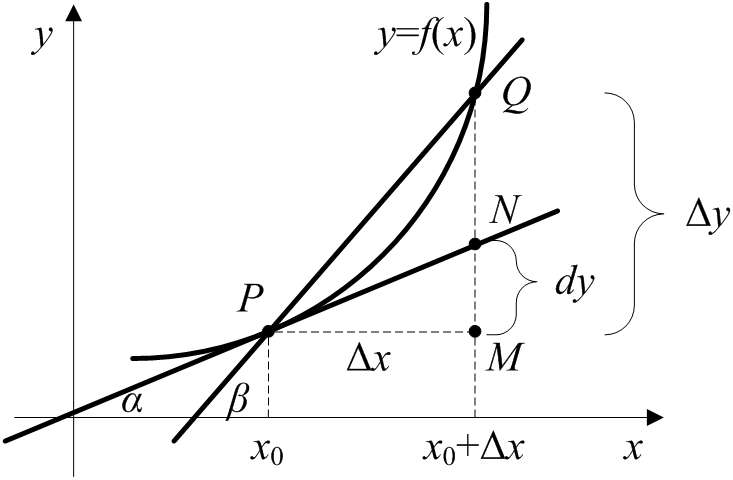
\includegraphics[height=4cm]{2.3.png}
\end{figure}

当{\it Q}点无穷逼近{\it P}的时候,即$\beta \rightarrow \alpha $,可得:
\[
\underset{\Delta x\rightarrow 0}{\lim}\Delta y=\underset{\Delta x\rightarrow 0}{\lim}\left( \tan \beta \cdot \Delta x \right) =\tan \alpha \cdot \Delta x=dy
\]
从几何上看,当{\it Q}点无穷逼近{\it P}的时候,线段{\it MQ}的长度无穷逼近线段{\it MN}的长度。
或者说,我们可以用线段{\it MQ}代替线段{\it MN},且线段{\it NQ}是可以被忽略的。
被忽略的{\it NQ}就是那个高阶无穷小量$o\left( \Delta x \right) $。

微分的几何意义是在一个微小的局部,我们可以用直线函数近似代替曲线函数,即“以直代曲”。
这种局部线性化的思想广泛应用于自然科学和工程。

%============================================================
\subsection{微分的物理应用}

用微分我们可以近似计算一些工程值。
若已知$f\left( x_0 \right) $,如何快速求$f\left( x_0+\Delta x \right) $处的值。
这类问题可以通过微分近似求解。当$\Delta x$足够小时,我们可以用$dy$代替$\Delta y$,从而有:
\[
y=f\left( x_0 \right) +\Delta y\approx f\left( x_0 \right) +dy
\]

~

\begin{example}
扩音器插头为一圆柱体,截面半径r=0.15cm,长l=4cm,为提高导电性,需要在该圆柱体侧面镀一层0.001cm的纯铜,问约需要多少。
\end{example}

解:

显然该问题就是估算体积的变化。
圆柱体体积:
\[
V=\pi r^2l
\]
侧面镀一层纯铜,相当于半径变化。
所用铜的体积等于由于半径的微小变化引起的圆柱体体积的微增量。
\[
dV=2\pi rl=2\pi \cdot 0.15\cdot 4\cdot 0.001=0.00377\mathrm{cm}^3
\]




